\documentclass[twoside]{book}

% Packages required by doxygen
\usepackage{fixltx2e}
\usepackage{calc}
\usepackage{doxygen}
\usepackage[export]{adjustbox} % also loads graphicx
\usepackage{graphicx}
\usepackage[utf8]{inputenc}
\usepackage{makeidx}
\usepackage{multicol}
\usepackage{multirow}
\PassOptionsToPackage{warn}{textcomp}
\usepackage{textcomp}
\usepackage[nointegrals]{wasysym}
\usepackage[table]{xcolor}

% Font selection
\usepackage[T1]{fontenc}
\usepackage[scaled=.90]{helvet}
\usepackage{courier}
\usepackage{amssymb}
\usepackage{sectsty}
\renewcommand{\familydefault}{\sfdefault}
\allsectionsfont{%
  \fontseries{bc}\selectfont%
  \color{darkgray}%
}
\renewcommand{\DoxyLabelFont}{%
  \fontseries{bc}\selectfont%
  \color{darkgray}%
}
\newcommand{\+}{\discretionary{\mbox{\scriptsize$\hookleftarrow$}}{}{}}

% Page & text layout
\usepackage{geometry}
\geometry{%
  a4paper,%
  top=2.5cm,%
  bottom=2.5cm,%
  left=2.5cm,%
  right=2.5cm%
}
\tolerance=750
\hfuzz=15pt
\hbadness=750
\setlength{\emergencystretch}{15pt}
\setlength{\parindent}{0cm}
\setlength{\parskip}{3ex plus 2ex minus 2ex}
\makeatletter
\renewcommand{\paragraph}{%
  \@startsection{paragraph}{4}{0ex}{-1.0ex}{1.0ex}{%
    \normalfont\normalsize\bfseries\SS@parafont%
  }%
}
\renewcommand{\subparagraph}{%
  \@startsection{subparagraph}{5}{0ex}{-1.0ex}{1.0ex}{%
    \normalfont\normalsize\bfseries\SS@subparafont%
  }%
}
\makeatother

% Headers & footers
\usepackage{fancyhdr}
\pagestyle{fancyplain}
\fancyhead[LE]{\fancyplain{}{\bfseries\thepage}}
\fancyhead[CE]{\fancyplain{}{}}
\fancyhead[RE]{\fancyplain{}{\bfseries\leftmark}}
\fancyhead[LO]{\fancyplain{}{\bfseries\rightmark}}
\fancyhead[CO]{\fancyplain{}{}}
\fancyhead[RO]{\fancyplain{}{\bfseries\thepage}}
\fancyfoot[LE]{\fancyplain{}{}}
\fancyfoot[CE]{\fancyplain{}{}}
\fancyfoot[RE]{\fancyplain{}{\bfseries\scriptsize Generated by Doxygen }}
\fancyfoot[LO]{\fancyplain{}{\bfseries\scriptsize Generated by Doxygen }}
\fancyfoot[CO]{\fancyplain{}{}}
\fancyfoot[RO]{\fancyplain{}{}}
\renewcommand{\footrulewidth}{0.4pt}
\renewcommand{\chaptermark}[1]{%
  \markboth{#1}{}%
}
\renewcommand{\sectionmark}[1]{%
  \markright{\thesection\ #1}%
}

% Indices & bibliography
\usepackage{natbib}
\usepackage[titles]{tocloft}
\setcounter{tocdepth}{3}
\setcounter{secnumdepth}{5}
\makeindex

% Hyperlinks (required, but should be loaded last)
\usepackage{ifpdf}
\ifpdf
  \usepackage[pdftex,pagebackref=true]{hyperref}
\else
  \usepackage[ps2pdf,pagebackref=true]{hyperref}
\fi
\hypersetup{%
  colorlinks=true,%
  linkcolor=blue,%
  citecolor=blue,%
  unicode%
}

% Custom commands
\newcommand{\clearemptydoublepage}{%
  \newpage{\pagestyle{empty}\cleardoublepage}%
}

\usepackage{caption}
\captionsetup{labelsep=space,justification=centering,font={bf},singlelinecheck=off,skip=4pt,position=top}

%===== C O N T E N T S =====

\begin{document}

% Titlepage & ToC
\hypersetup{pageanchor=false,
             bookmarksnumbered=true,
             pdfencoding=unicode
            }
\pagenumbering{alph}
\begin{titlepage}
\vspace*{7cm}
\begin{center}%
{\Large ag\+\_\+gen }\\
\vspace*{1cm}
{\large Generated by Doxygen 1.8.14}\\
\end{center}
\end{titlepage}
\clearemptydoublepage
\pagenumbering{roman}
\tableofcontents
\clearemptydoublepage
\pagenumbering{arabic}
\hypersetup{pageanchor=true}

%--- Begin generated contents ---
\chapter{Hierarchical Index}
\section{Class Hierarchy}
This inheritance list is sorted roughly, but not completely, alphabetically\+:\begin{DoxyCompactList}
\item \contentsline{section}{A\+G\+Gen}{\pageref{class_a_g_gen}}{}
\item \contentsline{section}{Asset}{\pageref{class_asset}}{}
\item \contentsline{section}{Asset\+Group}{\pageref{class_asset_group}}{}
\item \contentsline{section}{Attack\+\_\+\+Node}{\pageref{struct_attack___node}}{}
\item \contentsline{section}{Config}{\pageref{class_config}}{}
\item \contentsline{section}{Connection}{\pageref{class_connection}}{}
\item \contentsline{section}{DB}{\pageref{class_d_b}}{}
\item \contentsline{section}{Ed}{\pageref{struct_ed}}{}
\item \contentsline{section}{Edge}{\pageref{class_edge}}{}
\item \contentsline{section}{Encoded\+Quality}{\pageref{union_encoded_quality}}{}
\item \contentsline{section}{Encoded\+Topology}{\pageref{union_encoded_topology}}{}
\item \contentsline{section}{Exploit}{\pageref{class_exploit}}{}
\item \contentsline{section}{Factbase}{\pageref{class_factbase}}{}
\item \contentsline{section}{hashnode}{\pageref{structhashnode}}{}
\item \contentsline{section}{hashtable}{\pageref{structhashtable}}{}
\item \contentsline{section}{Keyvalue}{\pageref{class_keyvalue}}{}
\item \contentsline{section}{Network}{\pageref{class_network}}{}
\item \contentsline{section}{Network\+State}{\pageref{class_network_state}}{}
\item \contentsline{section}{Odometer}{\pageref{class_odometer}}{}
\item \contentsline{section}{Parameterized\+Quality}{\pageref{struct_parameterized_quality}}{}
\item \contentsline{section}{Parameterized\+Topology}{\pageref{class_parameterized_topology}}{}
\item \contentsline{section}{Quality}{\pageref{class_quality}}{}
\item runtime\+\_\+error\begin{DoxyCompactList}
\item \contentsline{section}{D\+B\+Exception}{\pageref{class_d_b_exception}}{}
\end{DoxyCompactList}
\item \contentsline{section}{statement}{\pageref{structstatement}}{}
\item \contentsline{section}{str\+\_\+array}{\pageref{structstr__array}}{}
\item \contentsline{section}{Topology}{\pageref{class_topology}}{}
\item \contentsline{section}{Ve}{\pageref{struct_ve}}{}
\end{DoxyCompactList}

\chapter{Class Index}
\section{Class List}
Here are the classes, structs, unions and interfaces with brief descriptions\+:\begin{DoxyCompactList}
\item\contentsline{section}{\mbox{\hyperlink{class_a_g_gen}{A\+G\+Gen}} }{\pageref{class_a_g_gen}}{}
\item\contentsline{section}{\mbox{\hyperlink{class_asset}{Asset}} }{\pageref{class_asset}}{}
\item\contentsline{section}{\mbox{\hyperlink{class_asset_group}{Asset\+Group}} }{\pageref{class_asset_group}}{}
\item\contentsline{section}{\mbox{\hyperlink{struct_attack___node}{Attack\+\_\+\+Node}} }{\pageref{struct_attack___node}}{}
\item\contentsline{section}{\mbox{\hyperlink{class_config}{Config}} }{\pageref{class_config}}{}
\item\contentsline{section}{\mbox{\hyperlink{class_connection}{Connection}} }{\pageref{class_connection}}{}
\item\contentsline{section}{\mbox{\hyperlink{class_d_b}{DB}} }{\pageref{class_d_b}}{}
\item\contentsline{section}{\mbox{\hyperlink{class_d_b_exception}{D\+B\+Exception}} }{\pageref{class_d_b_exception}}{}
\item\contentsline{section}{\mbox{\hyperlink{struct_ed}{Ed}} }{\pageref{struct_ed}}{}
\item\contentsline{section}{\mbox{\hyperlink{class_edge}{Edge}} }{\pageref{class_edge}}{}
\item\contentsline{section}{\mbox{\hyperlink{union_encoded_quality}{Encoded\+Quality}} }{\pageref{union_encoded_quality}}{}
\item\contentsline{section}{\mbox{\hyperlink{union_encoded_topology}{Encoded\+Topology}} }{\pageref{union_encoded_topology}}{}
\item\contentsline{section}{\mbox{\hyperlink{class_exploit}{Exploit}} }{\pageref{class_exploit}}{}
\item\contentsline{section}{\mbox{\hyperlink{class_factbase}{Factbase}} }{\pageref{class_factbase}}{}
\item\contentsline{section}{\mbox{\hyperlink{structhashnode}{hashnode}} }{\pageref{structhashnode}}{}
\item\contentsline{section}{\mbox{\hyperlink{structhashtable}{hashtable}} }{\pageref{structhashtable}}{}
\item\contentsline{section}{\mbox{\hyperlink{class_keyvalue}{Keyvalue}} }{\pageref{class_keyvalue}}{}
\item\contentsline{section}{\mbox{\hyperlink{class_network}{Network}} }{\pageref{class_network}}{}
\item\contentsline{section}{\mbox{\hyperlink{class_network_state}{Network\+State}} }{\pageref{class_network_state}}{}
\item\contentsline{section}{\mbox{\hyperlink{class_odometer}{Odometer}} }{\pageref{class_odometer}}{}
\item\contentsline{section}{\mbox{\hyperlink{struct_parameterized_quality}{Parameterized\+Quality}} }{\pageref{struct_parameterized_quality}}{}
\item\contentsline{section}{\mbox{\hyperlink{class_parameterized_topology}{Parameterized\+Topology}} }{\pageref{class_parameterized_topology}}{}
\item\contentsline{section}{\mbox{\hyperlink{class_quality}{Quality}} }{\pageref{class_quality}}{}
\item\contentsline{section}{\mbox{\hyperlink{structstatement}{statement}} }{\pageref{structstatement}}{}
\item\contentsline{section}{\mbox{\hyperlink{structstr__array}{str\+\_\+array}} }{\pageref{structstr__array}}{}
\item\contentsline{section}{\mbox{\hyperlink{class_topology}{Topology}} }{\pageref{class_topology}}{}
\item\contentsline{section}{\mbox{\hyperlink{struct_ve}{Ve}} }{\pageref{struct_ve}}{}
\end{DoxyCompactList}

\chapter{Class Documentation}
\hypertarget{class_a_g_gen}{}\section{A\+G\+Gen Class Reference}
\label{class_a_g_gen}\index{A\+G\+Gen@{A\+G\+Gen}}


{\ttfamily \#include $<$ag\+\_\+gen.\+h$>$}

\subsection*{Public Member Functions}
\begin{DoxyCompactItemize}
\item 
\mbox{\hyperlink{class_a_g_gen_aa7d90a88f555644912a5bc11fc54a029}{A\+G\+Gen}} (\mbox{\hyperlink{class_network}{Network}} \&net\+\_\+i)
\begin{DoxyCompactList}\small\item\em \mbox{\hyperlink{class_a_g_gen}{A\+G\+Gen}} Constructor. \end{DoxyCompactList}\item 
void \mbox{\hyperlink{class_a_g_gen_a0c95ee4d204aa3cc985570f9cf592c14}{generate}} ()
\begin{DoxyCompactList}\small\item\em Generate Attack Graph. \end{DoxyCompactList}\end{DoxyCompactItemize}


\subsection{Detailed Description}
\mbox{\hyperlink{class_a_g_gen}{A\+G\+Gen}} class Main generator class that stores state for the entire graph generation process 

\subsection{Constructor \& Destructor Documentation}
\mbox{\Hypertarget{class_a_g_gen_aa7d90a88f555644912a5bc11fc54a029}\label{class_a_g_gen_aa7d90a88f555644912a5bc11fc54a029}} 
\index{A\+G\+Gen@{A\+G\+Gen}!A\+G\+Gen@{A\+G\+Gen}}
\index{A\+G\+Gen@{A\+G\+Gen}!A\+G\+Gen@{A\+G\+Gen}}
\subsubsection{\texorpdfstring{A\+G\+Gen()}{AGGen()}}
{\footnotesize\ttfamily A\+G\+Gen\+::\+A\+G\+Gen (\begin{DoxyParamCaption}\item[{\mbox{\hyperlink{class_network}{Network}} \&}]{net\+\_\+i }\end{DoxyParamCaption})\hspace{0.3cm}{\ttfamily [explicit]}}



\mbox{\hyperlink{class_a_g_gen}{A\+G\+Gen}} Constructor. 

Constructor for generator.

Builds a generator for creating attack graphs.


\begin{DoxyParams}{Parameters}
{\em net\+\_\+i} & The network to build the attack graph for \\
\hline
\end{DoxyParams}


\subsection{Member Function Documentation}
\mbox{\Hypertarget{class_a_g_gen_a0c95ee4d204aa3cc985570f9cf592c14}\label{class_a_g_gen_a0c95ee4d204aa3cc985570f9cf592c14}} 
\index{A\+G\+Gen@{A\+G\+Gen}!generate@{generate}}
\index{generate@{generate}!A\+G\+Gen@{A\+G\+Gen}}
\subsubsection{\texorpdfstring{generate()}{generate()}}
{\footnotesize\ttfamily void A\+G\+Gen\+::generate (\begin{DoxyParamCaption}{ }\end{DoxyParamCaption})}



Generate Attack Graph. 

Generate attack graph.

Begins the generation process.

Begin the generation of the attack graph. The algorithm is as follows\+: \begin{DoxyVerb} 1. Fetch next factbase to expand from the frontier
 2. Fetch all exploits
 3. Loop over each exploit to determine if it is applicable.
     a. Fetch preconditions of the exploit
     b. Generate all permutations of assets using the Odometer utility
     c. Apply each permutation of the assets to the preconditions.
     d. Check if ALL generated preconditions are present in the current factbase.
 4a. If all preconditions are found, apply the matching asset group to the postconditions of the exploit.
 4b. If not all preconditions are found, break and continue checking with the next exploit.
 5. Push the new network state onto the frontier to be expanded later.\end{DoxyVerb}
 

The documentation for this class was generated from the following files\+:\begin{DoxyCompactItemize}
\item 
src/ag\+\_\+gen/ag\+\_\+gen.\+h\item 
src/ag\+\_\+gen/ag\+\_\+gen.\+cpp\end{DoxyCompactItemize}

\hypertarget{class_asset}{}\section{Asset Struct Reference}
\label{class_asset}\index{Asset@{Asset}}
\subsection*{Public Member Functions}
\begin{DoxyCompactItemize}
\item 
\mbox{\Hypertarget{class_asset_a988f61edbd7acb419206c4fa815ca5fa}\label{class_asset_a988f61edbd7acb419206c4fa815ca5fa}} 
{\bfseries Asset} (int iid, int netid, std\+::string nname)
\item 
\mbox{\Hypertarget{class_asset_a356396b8ac2d08f11cc4a22e32bab8a1}\label{class_asset_a356396b8ac2d08f11cc4a22e32bab8a1}} 
void {\bfseries fetch\+\_\+qualities} ()
\end{DoxyCompactItemize}
\subsection*{Static Public Member Functions}
\begin{DoxyCompactItemize}
\item 
\mbox{\Hypertarget{class_asset_ac5dcdf40f494198bd14fa853082f0c3d}\label{class_asset_ac5dcdf40f494198bd14fa853082f0c3d}} 
static std\+::vector$<$ \mbox{\hyperlink{class_asset}{Asset}} $>$ {\bfseries fetch\+\_\+all} (const std\+::string \&network)
\end{DoxyCompactItemize}
\subsection*{Public Attributes}
\begin{DoxyCompactItemize}
\item 
\mbox{\Hypertarget{class_asset_ac37173d6b01d7b8caa7bd786b8de2269}\label{class_asset_ac37173d6b01d7b8caa7bd786b8de2269}} 
std\+::string {\bfseries id}
\item 
\mbox{\Hypertarget{class_asset_a4d760fd5b921c34c0c0398441e73ea90}\label{class_asset_a4d760fd5b921c34c0c0398441e73ea90}} 
std\+::string {\bfseries network\+\_\+id}
\end{DoxyCompactItemize}


The documentation for this struct was generated from the following files\+:\begin{DoxyCompactItemize}
\item 
src/ag\+\_\+gen/asset.\+h\item 
src/tools/graphing\+\_\+db.\+cpp\item 
src/ag\+\_\+gen/asset.\+cpp\end{DoxyCompactItemize}

\hypertarget{class_asset_group}{}\section{Asset\+Group Class Reference}
\label{class_asset_group}\index{Asset\+Group@{Asset\+Group}}
\subsection*{Public Member Functions}
\begin{DoxyCompactItemize}
\item 
\mbox{\Hypertarget{class_asset_group_a65936c858735a3addd31645a23507281}\label{class_asset_group_a65936c858735a3addd31645a23507281}} 
{\bfseries Asset\+Group} (std\+::vector$<$ \mbox{\hyperlink{class_quality}{Quality}} $>$ hypo\+\_\+quals, std\+::vector$<$ \mbox{\hyperlink{class_topology}{Topology}} $>$ hypo\+\_\+topos, std\+::vector$<$ int $>$ pperm)
\item 
\mbox{\Hypertarget{class_asset_group_a9cc88c1017e56949c8745feda8a1fff9}\label{class_asset_group_a9cc88c1017e56949c8745feda8a1fff9}} 
std\+::vector$<$ int $>$ {\bfseries get\+\_\+perm} () const
\item 
\mbox{\Hypertarget{class_asset_group_a1bbe8cfd576153fa260912ecd3d87350}\label{class_asset_group_a1bbe8cfd576153fa260912ecd3d87350}} 
std\+::vector$<$ \mbox{\hyperlink{class_quality}{Quality}} $>$ {\bfseries get\+\_\+hypo\+\_\+quals} () const
\item 
\mbox{\Hypertarget{class_asset_group_afbcd1d749c5e87290e48b34b3da8b8ba}\label{class_asset_group_afbcd1d749c5e87290e48b34b3da8b8ba}} 
std\+::vector$<$ \mbox{\hyperlink{class_topology}{Topology}} $>$ {\bfseries get\+\_\+hypo\+\_\+topos} () const
\item 
\mbox{\Hypertarget{class_asset_group_a8a583644f47734240cd3d0d30240a5e1}\label{class_asset_group_a8a583644f47734240cd3d0d30240a5e1}} 
void {\bfseries print\+\_\+facts} ()
\item 
\mbox{\Hypertarget{class_asset_group_a00b4fba96d51e69a7f253e2e712c0555}\label{class_asset_group_a00b4fba96d51e69a7f253e2e712c0555}} 
void {\bfseries print\+\_\+group} ()
\end{DoxyCompactItemize}


The documentation for this class was generated from the following files\+:\begin{DoxyCompactItemize}
\item 
src/ag\+\_\+gen/assetgroup.\+h\item 
src/ag\+\_\+gen/assetgroup.\+cpp\end{DoxyCompactItemize}

\hypertarget{struct_attack___node}{}\section{Attack\+\_\+\+Node Struct Reference}
\label{struct_attack___node}\index{Attack\+\_\+\+Node@{Attack\+\_\+\+Node}}
\subsection*{Public Attributes}
\begin{DoxyCompactItemize}
\item 
\mbox{\Hypertarget{struct_attack___node_ae02f66fca60568ee833aa48412a7dd1c}\label{struct_attack___node_ae02f66fca60568ee833aa48412a7dd1c}} 
std\+::string {\bfseries factbase\+\_\+id}
\item 
\mbox{\Hypertarget{struct_attack___node_a0077c68abdb58675e3eca13d4d5a6b18}\label{struct_attack___node_a0077c68abdb58675e3eca13d4d5a6b18}} 
std\+::string {\bfseries fact}
\end{DoxyCompactItemize}


The documentation for this struct was generated from the following file\+:\begin{DoxyCompactItemize}
\item 
src/tools/graphing\+\_\+db.\+cpp\end{DoxyCompactItemize}

\hypertarget{class_config}{}\section{Config Class Reference}
\label{class_config}\index{Config@{Config}}
\subsection*{Public Member Functions}
\begin{DoxyCompactItemize}
\item 
\mbox{\Hypertarget{class_config_aabd4efaa4f4d31be866a8e949cbb6c5b}\label{class_config_aabd4efaa4f4d31be866a8e949cbb6c5b}} 
{\bfseries Config} (std\+::string filename)
\item 
\mbox{\Hypertarget{class_config_ac37fd0d76799e50720733d0a2b363c50}\label{class_config_ac37fd0d76799e50720733d0a2b363c50}} 
std\+::string {\bfseries operator\mbox{[}$\,$\mbox{]}} (const std\+::string \&q)
\item 
\mbox{\Hypertarget{class_config_a145fb48e8056b0f8f5ce92d6184e73f9}\label{class_config_a145fb48e8056b0f8f5ce92d6184e73f9}} 
void {\bfseries print} ()
\item 
\mbox{\Hypertarget{class_config_a6372005e420ed1f57f1f53db7acdd631}\label{class_config_a6372005e420ed1f57f1f53db7acdd631}} 
std\+::string {\bfseries db\+\_\+string} ()
\end{DoxyCompactItemize}


The documentation for this class was generated from the following files\+:\begin{DoxyCompactItemize}
\item 
src/ag\+\_\+gen/config.\+h\item 
src/ag\+\_\+gen/config.\+cpp\end{DoxyCompactItemize}

\hypertarget{class_connection}{}\section{Connection Class Reference}
\label{class_connection}\index{Connection@{Connection}}
\subsection*{Public Member Functions}
\begin{DoxyCompactItemize}
\item 
\mbox{\Hypertarget{class_connection_a001e4ac07b5d15f9f3c33e1684765c18}\label{class_connection_a001e4ac07b5d15f9f3c33e1684765c18}} 
{\bfseries Connection} (const std\+::string \&conninfo)
\item 
\mbox{\Hypertarget{class_connection_a7539a59b23a618070a1deaa1ec1362df}\label{class_connection_a7539a59b23a618070a1deaa1ec1362df}} 
bool {\bfseries is\+\_\+connected} ()
\item 
\mbox{\Hypertarget{class_connection_af09c0078822c549da757873444f5c745}\label{class_connection_af09c0078822c549da757873444f5c745}} 
std\+::vector$<$ Row $>$ {\bfseries exec} (const std\+::string \&sql)
\end{DoxyCompactItemize}


The documentation for this class was generated from the following file\+:\begin{DoxyCompactItemize}
\item 
src/util/db.\+h\end{DoxyCompactItemize}

\hypertarget{class_d_b}{}\section{DB Class Reference}
\label{class_d_b}\index{DB@{DB}}
\subsection*{Public Member Functions}
\begin{DoxyCompactItemize}
\item 
\mbox{\Hypertarget{class_d_b_a85e1861d1c6f7139219b7f20f7cf527e}\label{class_d_b_a85e1861d1c6f7139219b7f20f7cf527e}} 
{\bfseries DB} (const std\+::string \&conninfo)
\item 
\mbox{\Hypertarget{class_d_b_a7ed8fbfd78327deab6d5b7e4998c28de}\label{class_d_b_a7ed8fbfd78327deab6d5b7e4998c28de}} 
std\+::vector$<$ Row $>$ {\bfseries exec} (const std\+::string \&sql)
\end{DoxyCompactItemize}


The documentation for this class was generated from the following file\+:\begin{DoxyCompactItemize}
\item 
src/util/db.\+h\end{DoxyCompactItemize}

\hypertarget{class_d_b_exception}{}\section{D\+B\+Exception Class Reference}
\label{class_d_b_exception}\index{D\+B\+Exception@{D\+B\+Exception}}
Inheritance diagram for D\+B\+Exception\+:\begin{figure}[H]
\begin{center}
\leavevmode
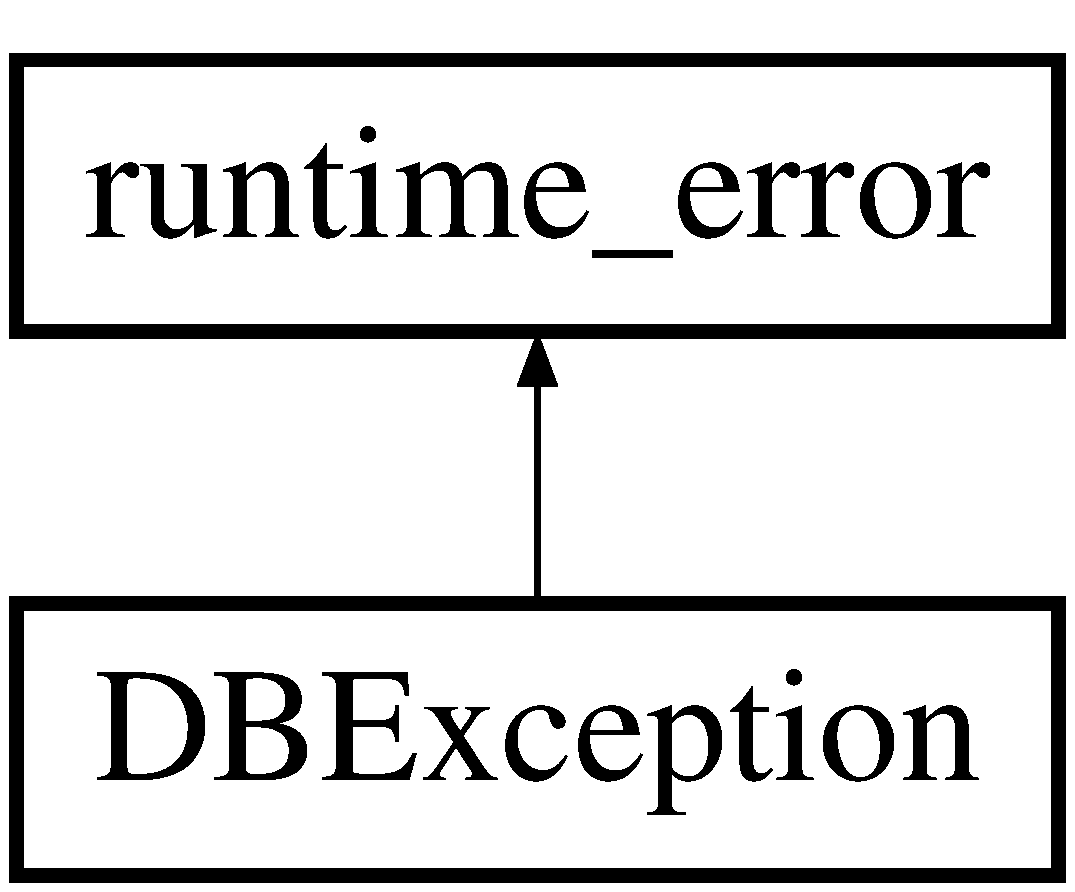
\includegraphics[height=2.000000cm]{class_d_b_exception}
\end{center}
\end{figure}
\subsection*{Public Member Functions}
\begin{DoxyCompactItemize}
\item 
\mbox{\Hypertarget{class_d_b_exception_a2257a50d74aa6ad59a80b3ba66cf63a1}\label{class_d_b_exception_a2257a50d74aa6ad59a80b3ba66cf63a1}} 
{\bfseries D\+B\+Exception} (std\+::string \&error\+\_\+message)
\item 
\mbox{\Hypertarget{class_d_b_exception_ad599de92924ae243175ca440423c9292}\label{class_d_b_exception_ad599de92924ae243175ca440423c9292}} 
{\bfseries D\+B\+Exception} (std\+::string \&\&error\+\_\+message)
\end{DoxyCompactItemize}


The documentation for this class was generated from the following file\+:\begin{DoxyCompactItemize}
\item 
src/util/db.\+h\end{DoxyCompactItemize}

\hypertarget{struct_ed}{}\section{Ed Struct Reference}
\label{struct_ed}\index{Ed@{Ed}}


The documentation for this struct was generated from the following file\+:\begin{DoxyCompactItemize}
\item 
src/examples/graph\+\_\+example.\+cpp\end{DoxyCompactItemize}

\hypertarget{class_edge}{}\section{Edge Struct Reference}
\label{class_edge}\index{Edge@{Edge}}
\subsection*{Public Member Functions}
\begin{DoxyCompactItemize}
\item 
\mbox{\Hypertarget{class_edge_a080dd300d092b097555aea558412482c}\label{class_edge_a080dd300d092b097555aea558412482c}} 
{\bfseries Edge} (int, int, \mbox{\hyperlink{class_exploit}{Exploit}} \&, \mbox{\hyperlink{class_asset_group}{Asset\+Group}} \&)
\item 
\mbox{\Hypertarget{class_edge_a869e88b1119a70b136f26a186203f49e}\label{class_edge_a869e88b1119a70b136f26a186203f49e}} 
void {\bfseries save} ()
\item 
\mbox{\Hypertarget{class_edge_a41de688b688ed7b033c683d0edd70d6f}\label{class_edge_a41de688b688ed7b033c683d0edd70d6f}} 
int {\bfseries get\+\_\+id} ()
\item 
\mbox{\Hypertarget{class_edge_a1798bd9da33a54c876f4a349b311d97e}\label{class_edge_a1798bd9da33a54c876f4a349b311d97e}} 
bool {\bfseries exists\+\_\+in\+\_\+db} ()
\end{DoxyCompactItemize}


The documentation for this struct was generated from the following files\+:\begin{DoxyCompactItemize}
\item 
src/ag\+\_\+gen/edge.\+h\item 
src/ag\+\_\+gen/edge.\+cpp\end{DoxyCompactItemize}

\hypertarget{union_encoded_quality}{}\section{Encoded\+Quality Union Reference}
\label{union_encoded_quality}\index{Encoded\+Quality@{Encoded\+Quality}}
\subsection*{Public Attributes}
\begin{DoxyCompactItemize}
\item 
\mbox{\Hypertarget{union_encoded_quality_ad06ef6dfc741c545d17702e1b4f41388}\label{union_encoded_quality_ad06ef6dfc741c545d17702e1b4f41388}} 
\begin{tabbing}
xx\=xx\=xx\=xx\=xx\=xx\=xx\=xx\=xx\=\kill
struct \{\\
\>int {\bfseries asset\_id}: 16\\
\>int {\bfseries attr}: 12\\
\>int {\bfseries op}: 4\\
\>int {\bfseries val}: 16\\
\} {\bfseries dec}\\

\end{tabbing}\item 
\mbox{\Hypertarget{union_encoded_quality_a1296310c98a4f422ae54260019a74873}\label{union_encoded_quality_a1296310c98a4f422ae54260019a74873}} 
size\+\_\+t {\bfseries enc}
\end{DoxyCompactItemize}


The documentation for this union was generated from the following file\+:\begin{DoxyCompactItemize}
\item 
src/ag\+\_\+gen/quality.\+h\end{DoxyCompactItemize}

\hypertarget{union_encoded_topology}{}\section{Encoded\+Topology Union Reference}
\label{union_encoded_topology}\index{Encoded\+Topology@{Encoded\+Topology}}
\subsection*{Public Attributes}
\begin{DoxyCompactItemize}
\item 
\mbox{\Hypertarget{union_encoded_topology_afaafcffae6ced53a27ab8a06745e1fef}\label{union_encoded_topology_afaafcffae6ced53a27ab8a06745e1fef}} 
\begin{tabbing}
xx\=xx\=xx\=xx\=xx\=xx\=xx\=xx\=xx\=\kill
struct \{\\
\>int {\bfseries from\_asset}: 16\\
\>int {\bfseries to\_asset}: 16\\
\>int {\bfseries dir}: 2\\
\>int {\bfseries property}: 10\\
\>int {\bfseries op}: 4\\
\>int {\bfseries value}: 16\\
\} {\bfseries dec}\\

\end{tabbing}\item 
\mbox{\Hypertarget{union_encoded_topology_a49d8caa1398285b6f0d57d963174705f}\label{union_encoded_topology_a49d8caa1398285b6f0d57d963174705f}} 
size\+\_\+t {\bfseries enc}
\end{DoxyCompactItemize}


The documentation for this union was generated from the following file\+:\begin{DoxyCompactItemize}
\item 
src/ag\+\_\+gen/topology.\+h\end{DoxyCompactItemize}

\hypertarget{class_exploit}{}\section{Exploit Class Reference}
\label{class_exploit}\index{Exploit@{Exploit}}
\subsection*{Public Member Functions}
\begin{DoxyCompactItemize}
\item 
\mbox{\Hypertarget{class_exploit_ab21f3b22cbe7a0913d790f0f0e813c51}\label{class_exploit_ab21f3b22cbe7a0913d790f0f0e813c51}} 
{\bfseries Exploit} (int pre\+Id, std\+::string \&pre\+Name, int pre\+Num\+Params)
\item 
\mbox{\Hypertarget{class_exploit_ad008d7b416105df2caa0f7394b0604a6}\label{class_exploit_ad008d7b416105df2caa0f7394b0604a6}} 
int {\bfseries get\+\_\+id} () const
\item 
\mbox{\Hypertarget{class_exploit_a33912e2531989534aa4558460aa0eac7}\label{class_exploit_a33912e2531989534aa4558460aa0eac7}} 
std\+::string {\bfseries get\+\_\+name} () const
\item 
\mbox{\Hypertarget{class_exploit_ad91d38497b04903abbaffbc7f3403062}\label{class_exploit_ad91d38497b04903abbaffbc7f3403062}} 
int {\bfseries get\+\_\+num\+\_\+params} () const
\item 
\mbox{\Hypertarget{class_exploit_a9320e46ddde5cd387703c470557449a6}\label{class_exploit_a9320e46ddde5cd387703c470557449a6}} 
void {\bfseries print\+\_\+preconds\+\_\+q} ()
\item 
\mbox{\Hypertarget{class_exploit_a509db4d9215f8c8f0a4964973376744a}\label{class_exploit_a509db4d9215f8c8f0a4964973376744a}} 
void {\bfseries print\+\_\+preconds\+\_\+t} ()
\item 
\mbox{\Hypertarget{class_exploit_aa90fccd79106107ea90ab6976b3b85d9}\label{class_exploit_aa90fccd79106107ea90ab6976b3b85d9}} 
void {\bfseries print\+\_\+postconds\+\_\+q} ()
\item 
\mbox{\Hypertarget{class_exploit_a2fc2e52ccadbf9d13340d2b0240a3112}\label{class_exploit_a2fc2e52ccadbf9d13340d2b0240a3112}} 
void {\bfseries print\+\_\+postconds\+\_\+t} ()
\item 
\mbox{\Hypertarget{class_exploit_a8fddb92a42f1144697234b249c62dbf6}\label{class_exploit_a8fddb92a42f1144697234b249c62dbf6}} 
void {\bfseries print\+\_\+id} ()
\item 
\mbox{\Hypertarget{class_exploit_a26590ba99ab5bb0ee087a0c3dcd1a48c}\label{class_exploit_a26590ba99ab5bb0ee087a0c3dcd1a48c}} 
std\+::vector$<$ \mbox{\hyperlink{struct_parameterized_quality}{Parameterized\+Quality}} $>$ {\bfseries precond\+\_\+list\+\_\+q} ()
\item 
\mbox{\Hypertarget{class_exploit_a430135c7ea3e331c2b1f1b277aed9278}\label{class_exploit_a430135c7ea3e331c2b1f1b277aed9278}} 
std\+::vector$<$ \mbox{\hyperlink{class_parameterized_topology}{Parameterized\+Topology}} $>$ {\bfseries precond\+\_\+list\+\_\+t} ()
\item 
\mbox{\Hypertarget{class_exploit_af72537cd66352048f9781f02abf4f7a0}\label{class_exploit_af72537cd66352048f9781f02abf4f7a0}} 
std\+::vector$<$ \mbox{\hyperlink{struct_parameterized_quality}{Parameterized\+Quality}} $>$ {\bfseries postcond\+\_\+list\+\_\+q} ()
\item 
\mbox{\Hypertarget{class_exploit_a09e724bafe4dfb7887cb007faf4aae8b}\label{class_exploit_a09e724bafe4dfb7887cb007faf4aae8b}} 
std\+::vector$<$ \mbox{\hyperlink{class_parameterized_topology}{Parameterized\+Topology}} $>$ {\bfseries postcond\+\_\+list\+\_\+t} ()
\end{DoxyCompactItemize}
\subsection*{Static Public Member Functions}
\begin{DoxyCompactItemize}
\item 
\mbox{\Hypertarget{class_exploit_a065f720bb655c3cd2419120dfb278423}\label{class_exploit_a065f720bb655c3cd2419120dfb278423}} 
static std\+::vector$<$ \mbox{\hyperlink{class_exploit}{Exploit}} $>$ {\bfseries fetch\+\_\+all} ()
\item 
\mbox{\Hypertarget{class_exploit_a9881ee99b10cf520d33b8039af28289c}\label{class_exploit_a9881ee99b10cf520d33b8039af28289c}} 
static void {\bfseries print\+\_\+all} ()
\end{DoxyCompactItemize}


The documentation for this class was generated from the following files\+:\begin{DoxyCompactItemize}
\item 
src/ag\+\_\+gen/exploit.\+h\item 
src/ag\+\_\+gen/exploit.\+cpp\end{DoxyCompactItemize}

\hypertarget{class_factbase}{}\section{Factbase Class Reference}
\label{class_factbase}\index{Factbase@{Factbase}}
\subsection*{Public Member Functions}
\begin{DoxyCompactItemize}
\item 
\mbox{\Hypertarget{class_factbase_ab8cee78aca6671002340a10985827f00}\label{class_factbase_ab8cee78aca6671002340a10985827f00}} 
void {\bfseries populate} ()
\item 
\mbox{\Hypertarget{class_factbase_ac71444bcc117054b8b6b6db0863cdce4}\label{class_factbase_ac71444bcc117054b8b6b6db0863cdce4}} 
void {\bfseries save} ()
\item 
\mbox{\Hypertarget{class_factbase_a448fd45ed66556fc226c7612b7b8cb43}\label{class_factbase_a448fd45ed66556fc226c7612b7b8cb43}} 
bool {\bfseries find\+\_\+quality} (\mbox{\hyperlink{class_quality}{Quality}} \&q) const
\item 
\mbox{\Hypertarget{class_factbase_a6d602fe105005cc65a005eb59ce7eb99}\label{class_factbase_a6d602fe105005cc65a005eb59ce7eb99}} 
bool {\bfseries find\+\_\+topology} (\mbox{\hyperlink{class_topology}{Topology}} \&t) const
\item 
\mbox{\Hypertarget{class_factbase_a99679712e07601eab5c127bd7b89d2ef}\label{class_factbase_a99679712e07601eab5c127bd7b89d2ef}} 
void {\bfseries add\+\_\+quality} (\mbox{\hyperlink{class_quality}{Quality}} \&q)
\item 
\mbox{\Hypertarget{class_factbase_a3b83acac4a0a1745bf443e743b4a4d56}\label{class_factbase_a3b83acac4a0a1745bf443e743b4a4d56}} 
void {\bfseries add\+\_\+topology} (\mbox{\hyperlink{class_topology}{Topology}} \&y)
\item 
\mbox{\Hypertarget{class_factbase_aef4739a4ad430207140ac08c70fc4296}\label{class_factbase_aef4739a4ad430207140ac08c70fc4296}} 
bool {\bfseries exists\+\_\+in\+\_\+db} ()
\item 
\mbox{\Hypertarget{class_factbase_a084a0040a84127a2f96cf153a7074fc6}\label{class_factbase_a084a0040a84127a2f96cf153a7074fc6}} 
void {\bfseries print} () const
\item 
\mbox{\Hypertarget{class_factbase_a2ee19922db4a6260a35417d1aa4dfcc2}\label{class_factbase_a2ee19922db4a6260a35417d1aa4dfcc2}} 
int {\bfseries get\+\_\+id} () const
\item 
\mbox{\Hypertarget{class_factbase_af88c3534ae74a4ea0f40b36ef1a48c9a}\label{class_factbase_af88c3534ae74a4ea0f40b36ef1a48c9a}} 
size\+\_\+t {\bfseries hash} () const
\end{DoxyCompactItemize}
\subsection*{Friends}
\begin{DoxyCompactItemize}
\item 
\mbox{\Hypertarget{class_factbase_af864ca38a6023b709224f8ceb6b37e9f}\label{class_factbase_af864ca38a6023b709224f8ceb6b37e9f}} 
class {\bfseries Network\+State}
\end{DoxyCompactItemize}


The documentation for this class was generated from the following files\+:\begin{DoxyCompactItemize}
\item 
src/ag\+\_\+gen/factbase.\+h\item 
src/ag\+\_\+gen/factbase.\+cpp\end{DoxyCompactItemize}

\hypertarget{structhashnode}{}\section{hashnode Struct Reference}
\label{structhashnode}\index{hashnode@{hashnode}}
\subsection*{Public Attributes}
\begin{DoxyCompactItemize}
\item 
\mbox{\Hypertarget{structhashnode_a96604523eefa545e20f706652f7b27ee}\label{structhashnode_a96604523eefa545e20f706652f7b27ee}} 
char $\ast$ {\bfseries key}
\item 
\mbox{\Hypertarget{structhashnode_aeeb288de3af1e422ea5c897f59cac8f2}\label{structhashnode_aeeb288de3af1e422ea5c897f59cac8f2}} 
void $\ast$ {\bfseries val}
\item 
\mbox{\Hypertarget{structhashnode_a5da30b694097f9b33085916bfef95067}\label{structhashnode_a5da30b694097f9b33085916bfef95067}} 
struct \mbox{\hyperlink{structhashnode}{hashnode}} $\ast$ {\bfseries next}
\end{DoxyCompactItemize}


The documentation for this struct was generated from the following file\+:\begin{DoxyCompactItemize}
\item 
src/util/hash.\+h\end{DoxyCompactItemize}

\hypertarget{structhashtable}{}\section{hashtable Struct Reference}
\label{structhashtable}\index{hashtable@{hashtable}}
\subsection*{Public Attributes}
\begin{DoxyCompactItemize}
\item 
\mbox{\Hypertarget{structhashtable_a9c06936411ea272cc8ac20b701d50b53}\label{structhashtable_a9c06936411ea272cc8ac20b701d50b53}} 
\mbox{\hyperlink{structhashnode}{hashnode}} $\ast$$\ast$ {\bfseries arr}
\item 
\mbox{\Hypertarget{structhashtable_ab62bd10297b090cfce7d728fd650e51d}\label{structhashtable_ab62bd10297b090cfce7d728fd650e51d}} 
int {\bfseries size}
\item 
\mbox{\Hypertarget{structhashtable_a8b6960345ca95dba2c9d4f9834b78972}\label{structhashtable_a8b6960345ca95dba2c9d4f9834b78972}} 
int {\bfseries used}
\end{DoxyCompactItemize}


The documentation for this struct was generated from the following file\+:\begin{DoxyCompactItemize}
\item 
src/util/hash.\+h\end{DoxyCompactItemize}

\hypertarget{class_keyvalue}{}\section{Keyvalue Class Reference}
\label{class_keyvalue}\index{Keyvalue@{Keyvalue}}
\subsection*{Public Member Functions}
\begin{DoxyCompactItemize}
\item 
\mbox{\Hypertarget{class_keyvalue_a292a85f63c2de771c8fa7d3b8a82e1be}\label{class_keyvalue_a292a85f63c2de771c8fa7d3b8a82e1be}} 
void {\bfseries populate} (std\+::vector$<$ std\+::string $>$ v)
\item 
\mbox{\Hypertarget{class_keyvalue_acaa4c8e2005fb9757e8cb584433401e5}\label{class_keyvalue_acaa4c8e2005fb9757e8cb584433401e5}} 
{\footnotesize template$<$typename U $>$ }\\std\+::enable\+\_\+if$<$ can\+\_\+get\+\_\+name$<$ U $>$\+::value, void $>$\+::type {\bfseries insert} (U \&target)
\item 
\mbox{\Hypertarget{class_keyvalue_a61c4aedfeb8b34525b954f893690e514}\label{class_keyvalue_a61c4aedfeb8b34525b954f893690e514}} 
{\footnotesize template$<$typename U $>$ }\\std\+::enable\+\_\+if$<$!can\+\_\+get\+\_\+name$<$ U $>$\+::value, void $>$\+::type {\bfseries insert} (U \&target)
\item 
\mbox{\Hypertarget{class_keyvalue_a6e50ffd83f7f1e5808072ab59d71147a}\label{class_keyvalue_a6e50ffd83f7f1e5808072ab59d71147a}} 
int {\bfseries operator\mbox{[}$\,$\mbox{]}} (const std\+::string \&str) const
\item 
\mbox{\Hypertarget{class_keyvalue_a02404a9180538efc9135180f28884336}\label{class_keyvalue_a02404a9180538efc9135180f28884336}} 
std\+::string {\bfseries operator\mbox{[}$\,$\mbox{]}} (int num) const
\item 
\mbox{\Hypertarget{class_keyvalue_a940e6119f94f943e6485ea1b7065882f}\label{class_keyvalue_a940e6119f94f943e6485ea1b7065882f}} 
int {\bfseries size} () const
\end{DoxyCompactItemize}


The documentation for this class was generated from the following file\+:\begin{DoxyCompactItemize}
\item 
src/util/keyvalue.\+h\end{DoxyCompactItemize}

\hypertarget{class_network}{}\section{Network Class Reference}
\label{class_network}\index{Network@{Network}}
\subsection*{Public Member Functions}
\begin{DoxyCompactItemize}
\item 
\mbox{\Hypertarget{class_network_a3cb970fdbad7e8156db8df8951bfb18a}\label{class_network_a3cb970fdbad7e8156db8df8951bfb18a}} 
{\bfseries Network} (std\+::string \&name)
\item 
\mbox{\Hypertarget{class_network_a979bd0fe04eba3b46e0bf6e03b53efd1}\label{class_network_a979bd0fe04eba3b46e0bf6e03b53efd1}} 
\mbox{\hyperlink{class_network_state}{Network\+State}} {\bfseries get\+\_\+initial\+\_\+state} ()
\item 
\mbox{\Hypertarget{class_network_a0da93244ee6aa2c51af37aa193481330}\label{class_network_a0da93244ee6aa2c51af37aa193481330}} 
int {\bfseries size} ()
\item 
\mbox{\Hypertarget{class_network_ac2dd899d3e405c04a7fcccac7ce0ac5d}\label{class_network_ac2dd899d3e405c04a7fcccac7ce0ac5d}} 
std\+::unique\+\_\+ptr$<$ \mbox{\hyperlink{class_network_state}{Network\+State}} $>$ {\bfseries generate\+\_\+network\+\_\+state} ()
\end{DoxyCompactItemize}
\subsection*{Public Attributes}
\begin{DoxyCompactItemize}
\item 
\mbox{\Hypertarget{class_network_a9d5dd21d0a010bb4fba5387d866880ac}\label{class_network_a9d5dd21d0a010bb4fba5387d866880ac}} 
\mbox{\hyperlink{class_keyvalue}{Keyvalue}} {\bfseries facts}
\end{DoxyCompactItemize}


The documentation for this class was generated from the following file\+:\begin{DoxyCompactItemize}
\item 
src/ag\+\_\+gen/network.\+h\end{DoxyCompactItemize}

\hypertarget{class_network_state}{}\section{Network\+State Class Reference}
\label{class_network_state}\index{Network\+State@{Network\+State}}
\subsection*{Public Member Functions}
\begin{DoxyCompactItemize}
\item 
\mbox{\Hypertarget{class_network_state_a1ab3020649c595c0158181a8603eceb0}\label{class_network_state_a1ab3020649c595c0158181a8603eceb0}} 
{\bfseries Network\+State} (\mbox{\hyperlink{class_network}{Network}} \&net)
\item 
\mbox{\Hypertarget{class_network_state_a201b7d2d98d68dac62121243f8a0b78f}\label{class_network_state_a201b7d2d98d68dac62121243f8a0b78f}} 
{\bfseries Network\+State} (const \mbox{\hyperlink{class_network_state}{Network\+State}} \&ns)
\item 
\mbox{\Hypertarget{class_network_state_af22d39ca80d818d3c15ff27bf2b9900b}\label{class_network_state_af22d39ca80d818d3c15ff27bf2b9900b}} 
const \mbox{\hyperlink{class_factbase}{Factbase}} \& {\bfseries get\+\_\+factbase} () const
\item 
\mbox{\Hypertarget{class_network_state_a0ac88601dc6b8263982c6a56c24d250e}\label{class_network_state_a0ac88601dc6b8263982c6a56c24d250e}} 
size\+\_\+t {\bfseries get\+\_\+hash} () const
\item 
\mbox{\Hypertarget{class_network_state_ae63be4f6d74a4f6f71da384434dba233}\label{class_network_state_ae63be4f6d74a4f6f71da384434dba233}} 
void {\bfseries add\+\_\+qualities} (std\+::vector$<$ \mbox{\hyperlink{class_quality}{Quality}} $>$ q)
\item 
\mbox{\Hypertarget{class_network_state_a96debade0210181e318f5dcb79847cf9}\label{class_network_state_a96debade0210181e318f5dcb79847cf9}} 
void {\bfseries add\+\_\+topologies} (std\+::vector$<$ \mbox{\hyperlink{class_topology}{Topology}} $>$ t)
\end{DoxyCompactItemize}
\subsection*{Friends}
\begin{DoxyCompactItemize}
\item 
\mbox{\Hypertarget{class_network_state_af57acf978b262397fa5d12d64b884bde}\label{class_network_state_af57acf978b262397fa5d12d64b884bde}} 
class {\bfseries Factbase}
\end{DoxyCompactItemize}


The documentation for this class was generated from the following files\+:\begin{DoxyCompactItemize}
\item 
src/ag\+\_\+gen/network\+\_\+state.\+h\item 
src/ag\+\_\+gen/network\+\_\+state.\+cpp\end{DoxyCompactItemize}

\hypertarget{class_odometer}{}\section{Odometer Class Reference}
\label{class_odometer}\index{Odometer@{Odometer}}
\subsection*{Public Member Functions}
\begin{DoxyCompactItemize}
\item 
\mbox{\Hypertarget{class_odometer_a01675e615335239ff37909d74fec57ce}\label{class_odometer_a01675e615335239ff37909d74fec57ce}} 
{\bfseries Odometer} (int in\+\_\+n, int in\+\_\+k)
\item 
\mbox{\Hypertarget{class_odometer_a182297f889f24d71a1cd3c954175007e}\label{class_odometer_a182297f889f24d71a1cd3c954175007e}} 
void {\bfseries print} ()
\item 
\mbox{\Hypertarget{class_odometer_abcba3abd2b2c04cb31ddd40c490b3093}\label{class_odometer_abcba3abd2b2c04cb31ddd40c490b3093}} 
unsigned long {\bfseries length} ()
\item 
\mbox{\Hypertarget{class_odometer_a7870a18bd060d8e4f6a2ff22bf54a326}\label{class_odometer_a7870a18bd060d8e4f6a2ff22bf54a326}} 
std\+::vector$<$ int $>$ {\bfseries next} ()
\item 
\mbox{\Hypertarget{class_odometer_a0e7acb1f11f004d8e5414d15b833ecd7}\label{class_odometer_a0e7acb1f11f004d8e5414d15b833ecd7}} 
const std\+::vector$<$ int $>$ \& {\bfseries operator\mbox{[}$\,$\mbox{]}} (int idx) const
\item 
\mbox{\Hypertarget{class_odometer_a2995d1d19b0d2d4d214b71dd49e153ef}\label{class_odometer_a2995d1d19b0d2d4d214b71dd49e153ef}} 
void {\bfseries reset} ()
\item 
\mbox{\Hypertarget{class_odometer_af63ecac3d0e869a9a20044238f5064bf}\label{class_odometer_af63ecac3d0e869a9a20044238f5064bf}} 
int {\bfseries perm\+\_\+length} ()
\item 
\mbox{\Hypertarget{class_odometer_a5c10257afd62f76109805c2ae426b443}\label{class_odometer_a5c10257afd62f76109805c2ae426b443}} 
std\+::vector$<$ std\+::vector$<$ int $>$ $>$ {\bfseries get\+\_\+all} ()
\end{DoxyCompactItemize}


The documentation for this class was generated from the following file\+:\begin{DoxyCompactItemize}
\item 
src/util/odometer.\+h\end{DoxyCompactItemize}

\hypertarget{struct_parameterized_quality}{}\section{Parameterized\+Quality Struct Reference}
\label{struct_parameterized_quality}\index{Parameterized\+Quality@{Parameterized\+Quality}}
\subsection*{Public Member Functions}
\begin{DoxyCompactItemize}
\item 
\mbox{\Hypertarget{struct_parameterized_quality_a2a240ab18ff1bdc683e7190b880b2e3f}\label{struct_parameterized_quality_a2a240ab18ff1bdc683e7190b880b2e3f}} 
int {\bfseries get\+\_\+param\+\_\+num} ()
\item 
\mbox{\Hypertarget{struct_parameterized_quality_ae9c8b5e97bac869232094bb2b42ab437}\label{struct_parameterized_quality_ae9c8b5e97bac869232094bb2b42ab437}} 
void {\bfseries print} ()
\end{DoxyCompactItemize}
\subsection*{Public Attributes}
\begin{DoxyCompactItemize}
\item 
\mbox{\Hypertarget{struct_parameterized_quality_a3f645eec66a463f0c16d22d85785235c}\label{struct_parameterized_quality_a3f645eec66a463f0c16d22d85785235c}} 
int {\bfseries param}
\item 
\mbox{\Hypertarget{struct_parameterized_quality_a041debe48f84184b94175c1e14ea755f}\label{struct_parameterized_quality_a041debe48f84184b94175c1e14ea755f}} 
std\+::string {\bfseries name}
\item 
\mbox{\Hypertarget{struct_parameterized_quality_ae169312cf2a4390fa5679e2725e8d7b3}\label{struct_parameterized_quality_ae169312cf2a4390fa5679e2725e8d7b3}} 
std\+::string {\bfseries value}
\end{DoxyCompactItemize}


The documentation for this struct was generated from the following files\+:\begin{DoxyCompactItemize}
\item 
src/ag\+\_\+gen/parameterized\+\_\+quality.\+h\item 
src/ag\+\_\+gen/parameterized\+\_\+quality.\+cpp\end{DoxyCompactItemize}

\hypertarget{class_parameterized_topology}{}\section{Parameterized\+Topology Class Reference}
\label{class_parameterized_topology}\index{Parameterized\+Topology@{Parameterized\+Topology}}
\subsection*{Public Member Functions}
\begin{DoxyCompactItemize}
\item 
\mbox{\Hypertarget{class_parameterized_topology_ae27f389dcb62b6605af912e7f01db34e}\label{class_parameterized_topology_ae27f389dcb62b6605af912e7f01db34e}} 
{\bfseries Parameterized\+Topology} (int from\+\_\+param, int to\+\_\+param, std\+::string \&dir, std\+::string \&prop, std\+::string \&op, std\+::string \&val)
\item 
\mbox{\Hypertarget{class_parameterized_topology_a29c2e73fe247051bb482f7b62ec69e07}\label{class_parameterized_topology_a29c2e73fe247051bb482f7b62ec69e07}} 
int {\bfseries get\+\_\+from\+\_\+param} ()
\item 
\mbox{\Hypertarget{class_parameterized_topology_a3731290eba71feec0e1dc328abbd3ccf}\label{class_parameterized_topology_a3731290eba71feec0e1dc328abbd3ccf}} 
int {\bfseries get\+\_\+to\+\_\+param} ()
\item 
\mbox{\Hypertarget{class_parameterized_topology_a3053c3fa69b92c37eee58aefce96a35f}\label{class_parameterized_topology_a3053c3fa69b92c37eee58aefce96a35f}} 
std\+::string {\bfseries get\+\_\+dir} ()
\item 
\mbox{\Hypertarget{class_parameterized_topology_a40d50bdba9284b71ad143967409314fb}\label{class_parameterized_topology_a40d50bdba9284b71ad143967409314fb}} 
std\+::string {\bfseries get\+\_\+property} ()
\item 
\mbox{\Hypertarget{class_parameterized_topology_ab3f13da35969abe7e676a248a55be891}\label{class_parameterized_topology_ab3f13da35969abe7e676a248a55be891}} 
std\+::string {\bfseries get\+\_\+operation} ()
\item 
\mbox{\Hypertarget{class_parameterized_topology_af2373d44e3d5b1f87498fe8fe5cabd74}\label{class_parameterized_topology_af2373d44e3d5b1f87498fe8fe5cabd74}} 
std\+::string {\bfseries get\+\_\+value} ()
\item 
\mbox{\Hypertarget{class_parameterized_topology_aa438a3cdaa7b02e9a1984d68bf676990}\label{class_parameterized_topology_aa438a3cdaa7b02e9a1984d68bf676990}} 
void {\bfseries print} ()
\end{DoxyCompactItemize}


The documentation for this class was generated from the following files\+:\begin{DoxyCompactItemize}
\item 
src/ag\+\_\+gen/parameterized\+\_\+topology.\+h\item 
src/ag\+\_\+gen/parameterized\+\_\+topology.\+cpp\end{DoxyCompactItemize}

\hypertarget{class_quality}{}\section{Quality Class Reference}
\label{class_quality}\index{Quality@{Quality}}
\subsection*{Public Member Functions}
\begin{DoxyCompactItemize}
\item 
\mbox{\Hypertarget{class_quality_aa432c0b241ca875576cc821f6a36f3ee}\label{class_quality_aa432c0b241ca875576cc821f6a36f3ee}} 
{\bfseries Quality} (int asset\+Id, std\+::string qual\+Name, std\+::string op, std\+::string qual\+Value)
\item 
\mbox{\Hypertarget{class_quality_a28dfd360831d210cd6c36885837036a0}\label{class_quality_a28dfd360831d210cd6c36885837036a0}} 
std\+::string {\bfseries get\+\_\+name} () const
\item 
\mbox{\Hypertarget{class_quality_a97187cfcac228c0cbbfdbc88ae28a6e7}\label{class_quality_a97187cfcac228c0cbbfdbc88ae28a6e7}} 
std\+::string {\bfseries get\+\_\+op} () const
\item 
\mbox{\Hypertarget{class_quality_ae1107bd1cefb13f3dd7d51e310ed784d}\label{class_quality_ae1107bd1cefb13f3dd7d51e310ed784d}} 
void {\bfseries print} () const
\item 
\mbox{\Hypertarget{class_quality_a9e2bdc66c0189feb5600fb4122bb99cf}\label{class_quality_a9e2bdc66c0189feb5600fb4122bb99cf}} 
\mbox{\hyperlink{union_encoded_quality}{Encoded\+Quality}} {\bfseries encode} (const \mbox{\hyperlink{class_keyvalue}{Keyvalue}} \&kv\+\_\+facts) const
\item 
\mbox{\Hypertarget{class_quality_a44c77630be5e4c6c6c1ed0beb6f9466a}\label{class_quality_a44c77630be5e4c6c6c1ed0beb6f9466a}} 
bool {\bfseries operator==} (const \mbox{\hyperlink{class_quality}{Quality}} \&rhs) const
\item 
\mbox{\Hypertarget{class_quality_a4b5934a7aa94a2423cd3ec2883a96d20}\label{class_quality_a4b5934a7aa94a2423cd3ec2883a96d20}} 
bool {\bfseries operator$<$} (const \mbox{\hyperlink{class_quality}{Quality}} \&rhs) const
\end{DoxyCompactItemize}
\subsection*{Static Public Member Functions}
\begin{DoxyCompactItemize}
\item 
\mbox{\Hypertarget{class_quality_a6e2adef9cad716b9496b5c0b94adfc1f}\label{class_quality_a6e2adef9cad716b9496b5c0b94adfc1f}} 
static std\+::vector$<$ \mbox{\hyperlink{class_quality}{Quality}} $>$ {\bfseries fetch\+\_\+all} ()
\item 
\mbox{\Hypertarget{class_quality_ac3454c44a6c0c9ab01e1fa74ddeb0b05}\label{class_quality_ac3454c44a6c0c9ab01e1fa74ddeb0b05}} 
static std\+::vector$<$ std\+::string $>$ {\bfseries fetch\+\_\+all\+\_\+attributes} ()
\item 
\mbox{\Hypertarget{class_quality_aeaf962a1b1d4b03f1f0f7b66a95c2e87}\label{class_quality_aeaf962a1b1d4b03f1f0f7b66a95c2e87}} 
static std\+::vector$<$ std\+::string $>$ {\bfseries fetch\+\_\+all\+\_\+values} ()
\end{DoxyCompactItemize}
\subsection*{Friends}
\begin{DoxyCompactItemize}
\item 
\mbox{\Hypertarget{class_quality_af57acf978b262397fa5d12d64b884bde}\label{class_quality_af57acf978b262397fa5d12d64b884bde}} 
class {\bfseries Factbase}
\end{DoxyCompactItemize}


The documentation for this class was generated from the following files\+:\begin{DoxyCompactItemize}
\item 
src/ag\+\_\+gen/quality.\+h\item 
src/ag\+\_\+gen/quality.\+cpp\end{DoxyCompactItemize}

\hypertarget{structstatement}{}\section{statement Struct Reference}
\label{structstatement}\index{statement@{statement}}
\subsection*{Public Attributes}
\begin{DoxyCompactItemize}
\item 
\mbox{\Hypertarget{structstatement_aa59b1ce6cc7019d377f53654a0523370}\label{structstatement_aa59b1ce6cc7019d377f53654a0523370}} 
char $\ast$ {\bfseries obj}
\item 
\mbox{\Hypertarget{structstatement_a9e68b6f394988603850ad2c279da4261}\label{structstatement_a9e68b6f394988603850ad2c279da4261}} 
char $\ast$ {\bfseries op}
\item 
\mbox{\Hypertarget{structstatement_a04e465c77c360274d45b38db2946cd4c}\label{structstatement_a04e465c77c360274d45b38db2946cd4c}} 
char $\ast$ {\bfseries val}
\end{DoxyCompactItemize}


The documentation for this struct was generated from the following file\+:\begin{DoxyCompactItemize}
\item 
src/util/build\+\_\+sql.\+h\end{DoxyCompactItemize}

\hypertarget{structstr__array}{}\section{str\+\_\+array Struct Reference}
\label{structstr__array}\index{str\+\_\+array@{str\+\_\+array}}
\subsection*{Public Attributes}
\begin{DoxyCompactItemize}
\item 
\mbox{\Hypertarget{structstr__array_a19242a7c35c6e1313f7499c51051ed9a}\label{structstr__array_a19242a7c35c6e1313f7499c51051ed9a}} 
char $\ast$$\ast$ {\bfseries arr}
\item 
\mbox{\Hypertarget{structstr__array_ac668db01aa69290943b464e74ec49897}\label{structstr__array_ac668db01aa69290943b464e74ec49897}} 
size\+\_\+t {\bfseries size}
\item 
\mbox{\Hypertarget{structstr__array_a10a3614f5d66821cf9c3b7be30edc854}\label{structstr__array_a10a3614f5d66821cf9c3b7be30edc854}} 
size\+\_\+t {\bfseries used}
\end{DoxyCompactItemize}


The documentation for this struct was generated from the following file\+:\begin{DoxyCompactItemize}
\item 
src/util/str\+\_\+array.\+h\end{DoxyCompactItemize}

\hypertarget{class_topology}{}\section{Topology Struct Reference}
\label{class_topology}\index{Topology@{Topology}}
\subsection*{Public Member Functions}
\begin{DoxyCompactItemize}
\item 
\mbox{\Hypertarget{class_topology_a367d6baa1a28bb910ee1e4a5e9efce6f}\label{class_topology_a367d6baa1a28bb910ee1e4a5e9efce6f}} 
{\bfseries Topology} (int f\+\_\+asset, int t\+\_\+asset, std\+::string dir, std\+::string property, std\+::string op, std\+::string val)
\item 
\mbox{\Hypertarget{class_topology_a831312276b8a62f0713c9fce1dfdeec7}\label{class_topology_a831312276b8a62f0713c9fce1dfdeec7}} 
int {\bfseries get\+\_\+from\+\_\+asset\+\_\+id} () const
\item 
\mbox{\Hypertarget{class_topology_a63d4535c6f1f7810b120f7f8dbdb8d00}\label{class_topology_a63d4535c6f1f7810b120f7f8dbdb8d00}} 
int {\bfseries get\+\_\+to\+\_\+asset\+\_\+id} () const
\item 
\mbox{\Hypertarget{class_topology_a6d75d298f9f9d7e7aafaedd8f479251f}\label{class_topology_a6d75d298f9f9d7e7aafaedd8f479251f}} 
std\+::string {\bfseries get\+\_\+property} () const
\item 
\mbox{\Hypertarget{class_topology_a8da83f454b9886e0eedfd4ea5e82eb46}\label{class_topology_a8da83f454b9886e0eedfd4ea5e82eb46}} 
std\+::string {\bfseries get\+\_\+op} () const
\item 
\mbox{\Hypertarget{class_topology_a84e1f54ba7ab7826ae0f236293d426d2}\label{class_topology_a84e1f54ba7ab7826ae0f236293d426d2}} 
std\+::string {\bfseries get\+\_\+value} () const
\item 
\mbox{\Hypertarget{class_topology_ab36ac813d1685f5bb8138785b2f20b9a}\label{class_topology_ab36ac813d1685f5bb8138785b2f20b9a}} 
std\+::string {\bfseries get\+\_\+dir} () const
\item 
\mbox{\Hypertarget{class_topology_a98fb8fa8b2a696a60a78a9ce6e5cb716}\label{class_topology_a98fb8fa8b2a696a60a78a9ce6e5cb716}} 
void {\bfseries print} () const
\item 
\mbox{\Hypertarget{class_topology_af4d5d8d0c349f0d9fe421be0d5fa4ff4}\label{class_topology_af4d5d8d0c349f0d9fe421be0d5fa4ff4}} 
const \mbox{\hyperlink{union_encoded_topology}{Encoded\+Topology}} {\bfseries encode} (const \mbox{\hyperlink{class_keyvalue}{Keyvalue}} \&kv\+\_\+facts) const
\item 
\mbox{\Hypertarget{class_topology_a92d55881f0d66806a1b0a6d895818eb1}\label{class_topology_a92d55881f0d66806a1b0a6d895818eb1}} 
bool {\bfseries operator==} (const \mbox{\hyperlink{class_topology}{Topology}} \&rhs) const
\item 
\mbox{\Hypertarget{class_topology_a504373f784b2364dd868fba9899754db}\label{class_topology_a504373f784b2364dd868fba9899754db}} 
bool {\bfseries operator$<$} (const \mbox{\hyperlink{class_topology}{Topology}} \&rhs) const
\end{DoxyCompactItemize}
\subsection*{Static Public Member Functions}
\begin{DoxyCompactItemize}
\item 
\mbox{\Hypertarget{class_topology_a3f71c740d529d715f81f93ac0fff11c9}\label{class_topology_a3f71c740d529d715f81f93ac0fff11c9}} 
static std\+::vector$<$ \mbox{\hyperlink{class_topology}{Topology}} $>$ {\bfseries fetch\+\_\+all} ()
\item 
\mbox{\Hypertarget{class_topology_a4ef79a34c2756a64daf40024d0f14f8f}\label{class_topology_a4ef79a34c2756a64daf40024d0f14f8f}} 
static std\+::vector$<$ std\+::string $>$ {\bfseries fetch\+\_\+all\+\_\+attributes} ()
\item 
\mbox{\Hypertarget{class_topology_ad726048461aaf6a1c15a7995d70a69ca}\label{class_topology_ad726048461aaf6a1c15a7995d70a69ca}} 
static std\+::vector$<$ std\+::string $>$ {\bfseries fetch\+\_\+all\+\_\+values} ()
\end{DoxyCompactItemize}
\subsection*{Public Attributes}
\begin{DoxyCompactItemize}
\item 
\mbox{\Hypertarget{class_topology_a82a3df76bc548b4c91325ad7cd3ced5d}\label{class_topology_a82a3df76bc548b4c91325ad7cd3ced5d}} 
std\+::string {\bfseries option}
\end{DoxyCompactItemize}
\subsection*{Friends}
\begin{DoxyCompactItemize}
\item 
\mbox{\Hypertarget{class_topology_af57acf978b262397fa5d12d64b884bde}\label{class_topology_af57acf978b262397fa5d12d64b884bde}} 
class {\bfseries Factbase}
\end{DoxyCompactItemize}


The documentation for this struct was generated from the following files\+:\begin{DoxyCompactItemize}
\item 
src/ag\+\_\+gen/topology.\+h\item 
src/tools/graphing\+\_\+db.\+cpp\item 
src/ag\+\_\+gen/topology.\+cpp\end{DoxyCompactItemize}

\hypertarget{struct_ve}{}\section{Ve Struct Reference}
\label{struct_ve}\index{Ve@{Ve}}
\subsection*{Public Attributes}
\begin{DoxyCompactItemize}
\item 
\mbox{\Hypertarget{struct_ve_afee989787cac3868f33c533774d00cd3}\label{struct_ve_afee989787cac3868f33c533774d00cd3}} 
std\+::string {\bfseries name}
\end{DoxyCompactItemize}


The documentation for this struct was generated from the following file\+:\begin{DoxyCompactItemize}
\item 
src/examples/graph\+\_\+example.\+cpp\end{DoxyCompactItemize}

%--- End generated contents ---

% Index
\backmatter
\newpage
\phantomsection
\clearemptydoublepage
\addcontentsline{toc}{chapter}{Index}
\printindex

\end{document}
